\graphicspath{ {./images/} }
\section{Operation of the System}

\subsection{Searching for Conversations}

\todo{1st priority: for @kq: use images to describe how a user uses the system. each image has a caption, in the text expand upon the caption. give a "fake" case study, the user first enters a query, then they look through conversations, then they do blah... etc.}

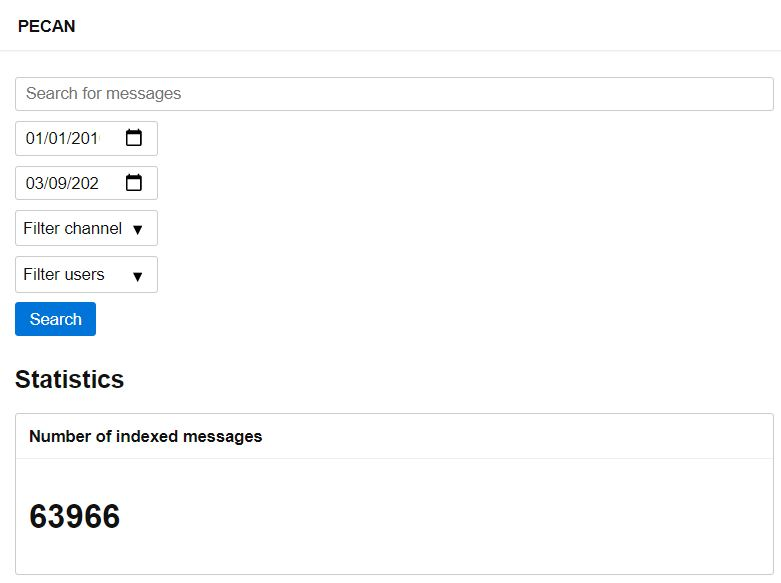
\includegraphics[scale=0.2]{homepage}

This is the homepage of the system.
\bigbreak

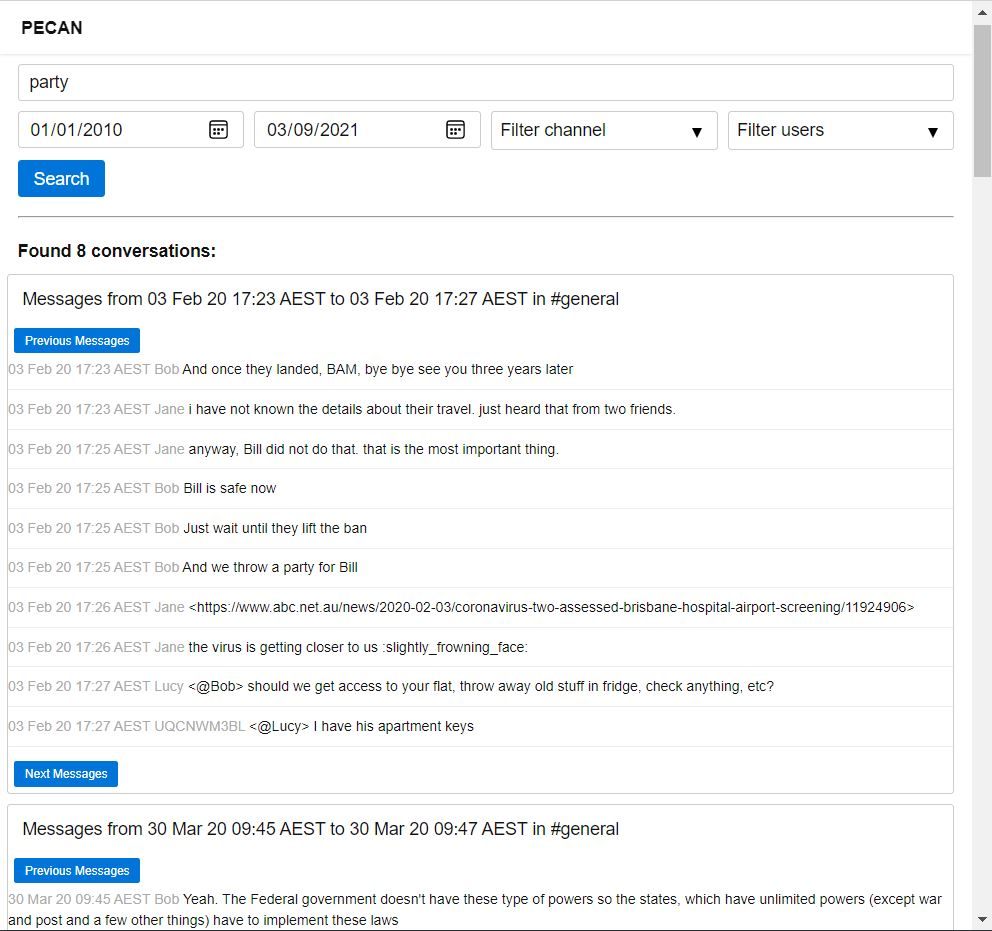
\includegraphics[scale=0.2]{searching}

Searching for converstaions with query "party".
\bigbreak

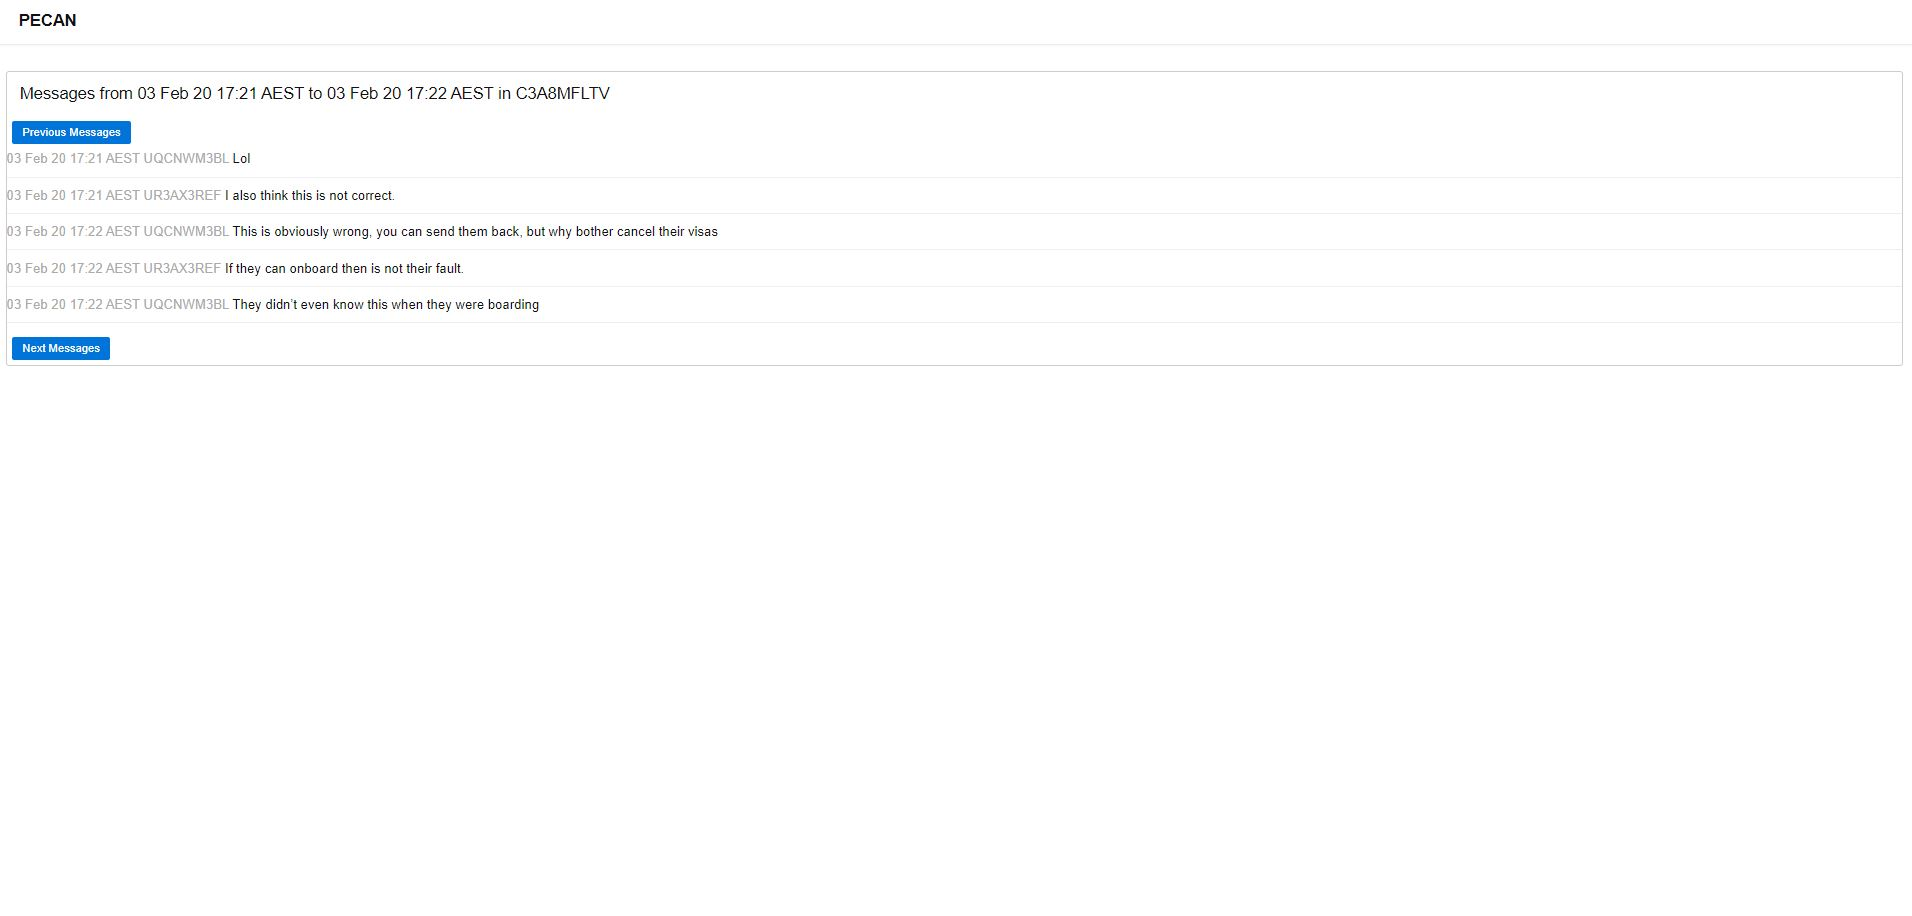
\includegraphics[scale=0.2]{traversing}

Traversing previous or next messages by clicking "previous messages" or "next messages".
\bigbreak

\subsection{System Implementation}
In this project, we use Go Language to implement the backend part of the system. We use elastic 7.0 as our serach engine. The elastic search provides a go module so that we can import and use it. The retrieval model we use to score messages is BM25. The score of each conversation is simply the sum of the scores of messages in that conversation. The retrieved conversations are merged and than ranked based on their scores. Users can access the system by searching with queries through an interface. The system will return conversations that are related to the query. After getting all the conversations, users can traversing through messages that come before and after each conversation.

\subsubsection{Conversation Aggregation}
There are many ways to retrieve conversations instead of messages. In this project we find conversations based on original messages. When we get a message, we define the five nearest messages before this message and five nearest messages after this message to be in the same conversation with this target message. We can retrieve these messages very easily with elastic search. These messages are then combined as one conversation. After retrieving all the conversations we want, we merge conversations that have identical messages. After merging conversations, we rank them by the sum of the scores of messages they have using quicksort. Normally, merged conversations are ranked higher than original conversations. Below is the pseudocode of the algorithm.

\begin{algorithm}
	\SetAlgoLined
	\caption{Retrieve Conversations}
	\SetKwInOut{Input}{inputs}
	\SetKwInOut{Output}{output}
	\SetKwProg{CreateConversations}{CreateConversations}{}{}
	\CreateConversations{$(Messages)$}{
		\Input{$messages$}
		\Output{$conversations$}
		$conversations \gets []$\\
		$i \gets 0$\\
		\ForEach{$message \in messages$}{
			$conversation \gets getSurroundingMessages(message$)\\
			$conversations[i] \gets conversation$\\
		}
		\Return{rankConversations(mergeConversations($conversations$))}
	}
\end{algorithm}
		
\subsubsection{Conversation Scoring}

\todo{3rd priority: for @kq: describe algorithms: mergeConversations, rankConversations}
To merge the conversations we retrieved, we simply go through every conversation. Since different conversations may have different channels, we keep an index for each channel so that we don't merge conversations with different channels together. We store the merged conversations into an array and for each channel, we save the index of the last conversation of the same channel in a map. Therefore, for each conversation, we can look for it's previous conversation with the same channel and check if they are overlapped. If they are overlapped we merge them and replace the old conversation on the index with the new conversation. Otherwise we insert the new conversation into the array and update the index for that channel.

\begin{algorithm}
	\SetAlgoLined
	\caption{Merge Conversations}
	\SetKwInOut{Input}{inputs}
	\SetKwInOut{Output}{output}
	\SetKwProg{MergeConversations}{MergeConversations}{}{}
	\MergeConversations{$(Messages)$}{
		\Input{$conversations$}
		\Output{$C$}
		$C \gets []$\\
		$H \gets HashMap$\\
		\ForEach{$conversation \in conversations$}{
			$index \gets H.get(conversation[0].Channel)$\\
			\If{$index \neq null$ and $conversation[0].Timestamp >= 	C[index][len(C[index])-1].Timestamp$}{
				\ForEach{$message \in conversation$}{
					\If{$message.Timestamp < C[index][len(C[index])-1].Timestamp$}{
							$C[index].append(message)$
					}
					\ElseIf{$message.Score>0$}{
						\ForEach{$keyMessage \in C[index]$}{
							\If{$keyMessage.Timestamp == message.Timestamp$ AND $keyMessage.Text==message.Text$}{
									$keyMessage \gets message$
							}
						}
					}
				}
			}
			\Else{
				$C.append(conversation)$
				$H[conversation[0].Channel] = len(C) -1$
			}
		}
		\Return{$C$}
	}
\end{algorithm}


\subsection{Running a User Study}

\todo{for @hs: description for how to use PECAN in a user study, how to use query logging, interaction logging.}

\subsection{Batch Evaluation}

\todo{for @hs}

\subsection{Planned Features}

\todo{4th priority: for @kq: channel filtering (in search time), filter by author, attachment search}